\documentclass[10pt]{exam}
\usepackage[hon]{template-for-exam}
\usepackage{endnotes,graphicx}
\usepackage{tikz,graphicx,enumitem,multicol,float,my-tikz-clipart,silence,cclicenses}
\graphicspath{{./figures/}}
\WarningFilter{latex}{Label `part}
\WarningFilter{latex}{There were multiply-defined labels}

\footer{}{\thepage}{\sc \myclass}


%\def\answer#1{\footnotetext{#1}}
%\def\myquestion{\item\stepcounter{footnote}}

\def\enoteheading{}
\def\answer#1{\endnotetext{#1}}
\def\theanswers{\theendnotes}
\def\myquestion{\item\stepcounter{endnote}}

\newenvironment{myquestions}{
  \begin{multicols*}{2}\begin{enumerate}
}{
  \end{enumerate}\end{multicols*}
}
\makeatletter
\patchcmd{\enit@setresumekeys}{\def}{\gdef}{}{}
\patchcmd{\enit@setresumekeys}{\def}{\gdef}{}{}
\makeatother

\newcommand{\myheading}[1]{\uplevel{\section*{#1}}
}
\newcommand{\mysubheading}[1]{\uplevel{\subsection*{#1}}
}

%uncomment if running Pandoc
% \renewcommand{\myheading}[1]{{\section*{#1}}}
% \renewcommand{\mysubheading}[1]{\subsection*{#1}}



%%%%%%%%%%%%%%%% Dates %%%%%%%%%%%%%%%%%%%
\def\quizday{Tue, Feb 10} % also used as HW Check A Day
\def\testday{Tue, Feb 24}

\def\one{Fri, Jan 30}
\def\two{Mon, Feb 2}
\def\three{Fri, Feb 6}
\def\four{Mon, Feb 9}
\def\five{We-Th, Feb 11-12}
\def\six{Fri, Feb 13}
%%%%%%%%%%%%%%%%%%%%%%%%%%%%%%%%%%%%%%%%%



\def\mytitle{Chapter 10 Homework (Rotational Motion)}
\title{\mytitle}
\date{\today}

\def\mymaketitle{
  \begin{flushleft}
    {\LARGE \textbf \mytitle \par}
  \end{flushleft}
}

\newcommand{\bs}[2]{\textbf{#1} (\sc #2 Points)}


\newcommand{\GFig}[2]{  
  \begin{figure}[H]
    \centering
    \includegraphics[width=#2]{08_#1_Figure.jpg}
    \caption{Giancolli Figure 8-#1.}
    \label{8-#1}
  \end{figure}
}


\begin{document}
\maketitle


\begin{center}
  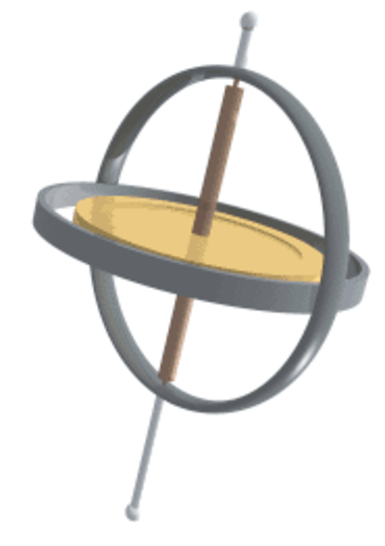
\includegraphics[height=6cm]{gyroscope.pdf}
\end{center}

\section*{HW Check A (collected on \quizday)}


%%%%%%%%%%%

\subsection*{Reading}

Please read the following on your own in the OpenStax textbook by the dates given.  It will give good context for class discussion.  Check off when you have completed them.

\vspace{1em}

\begin{checkboxes}
  \choice 6.1 (Review) Rotation Angle \& Angular Velocity \dotfill \one
  \choice 10.1 Angular Acceleration \dotfill \one
  \choice 10.2 Kinematics of Rotational Motion \dotfill \two
  \choice 9.2 The Second Condition of Equilibrium (definition of torque) \dotfill \three
\end{checkboxes}


\subsection*{Problems and Conceptual Question}


Get stamps from your instructor as you complete each of the following problems.  The conceptual questions (CQ) require at least one sentence of explanation.

\vspace{1em}

\noindent
{\sc Stamps will not be given if work is not shown on a separate sheet of paper}

\vspace{1em}


\begin{tabular}{|*{3}{p{4.8cm}|}}
  \hline
  %
  \bs{Ang. Quantities}{8}               
                    & \bs{Rot. Kin. Eqs.}{4}
                                      & \bs{Torque}{3}  \\
  Problems \#\ref{1p-i}-\ref{1p-f}
              & Problems \#\ref{2p-i}-\ref{2p-f} 
                    & Problems \#\ref{3p-i}-\ref{3p-f}\\
  Conceptual \#\ref{1q-i}-\ref{1q-f}
          & %Conceptual \#\ref{2q-i}-\ref{2q-f}
              & Conceptual \#\ref{3q-i}-\ref{3q-f} \\
          & \textbf{HW Quiz on \quizday} & \\[4em]\hline  
  %%
\end{tabular}



\pagebreak

\newcommand{\refsheet}{
  \section*{Selected Answers}

  \renewcommand{\enotesize}{\normalsize}
  \renewcommand{\enoteformat}{%
    \leftskip=1.8em
    \makebox[0pt][r]{\theenmark. }%
  }

  \hfill
  \theanswers
}

\refsheet
 
\pagebreak


\noindent
Questions and figures are from OpenStax \emph{College Physics}, 2nd ed, (Chapter 10) or Giancolli \emph{Physics: Principles with Applications}, 7th ed, (Chapter 8) unless otherwise noted.
 unless otherwise noted.



\begin{myquestions}

\myheading{Angular Quantites}
\mysubheading{Problems}



\myquestion (Giancoli P14) \label{1p-f}
A 61-cm-diameter wheel accelerates uniformly about its center from 120~rpm to 280~rpm in 4.0~s. Determine (a) its angular acceleration, and (b) the radial and tangential components of the linear acceleration of a point on the edge of the wheel 2.0~s after it has started accelerating. 
\answer{$\alpha = \SI{4.2}{\radian\per\second^2}$; 
      $a_C = \SI{134}{\meter\per\second^2}$;  
      $a_T = \SI{1.3}{\meter\per\second^2}$}


\myquestion (Original Question)
A turntable of radius 45~cm is turned by a circular rubber roller of radius 2.0~cm in contact with it at their outer edges (see Figure~\ref{turntables}).  The two wheels do not slip past each other If the small roller has an angular velocity of 35~rad/s, what is the angular velocity of the large turntable? \answer{1.56~rad/s}


\mysubheading{Conceptual Questions}

\myquestion (Giancoli MC1, modified) \label{1q-f}
Bonnie sits on the outer rim of a merry-go-round, and Jill sits midway between the center and the rim. The merry-go-round makes one complete revolution every 2~seconds. Who (if either) has the larger $v$ and who (if either) has the larger $\omega$?
\answer{Bonnie has larger $v$; they have the same $\omega$}



\myheading{Rotational Kinematic Equations}
\mysubheading{Problems}

\myquestion (P7) 
A gyroscope slows from an initial rate of 32.0~rad/s at a rate of \SI{0.700}{rad/s^2}. (a) How long does it take to come to rest?
(b) How many revolutions does it make before stopping?
\answer{(a) 45.7~s; (b) 116~rev}


\myquestion (Giancoli MC4) \label{3q-i}
The solid dot shown in Figure~\ref{8-36} is a pivot point. The board can rotate about the pivot. Which force shown exerts the largest magnitude torque on the board?
\answer{(c)}

\GFig{36}{6.5cm}
\myquestion (P14) 
Suppose you exert a force of 180 N tangential to a 0.280-m-radius 75.0-kg grindstone (a solid disk).(a) What torque is exerted? (b) What is the angular acceleration assuming negligible opposing friction? 
\answer{(a) \SI{50.4}{m.N}; (b) \SI{17.1}{rad/s^2}}



\mysubheading{Conceptual Questions}


\myquestion (Giancoli CQ12) \label{5q-f}
A sphere and a cylinder have the same radius and the same mass. They start from rest at the top of an incline.
(a) Which reaches the bottom first?
(b) Which has the greater speed at the bottom?
(c) Which has the greater total kinetic energy at the bottom?
(d) Which has the greater rotational kinetic energy?
\answer{(a) sphere; (b) sphere; (c) equal; (d) cylinder}



\myquestion (Giancoli P65) \label{6p-f}
A figure skater can increase her spin rotation rate from an initial state of 1.0~rev every 1.5~s to a final rate of 2.5~rev/s.  If her initial moment of inertia is \SI{4.6}{kg.m^2}, what is her final moment of inertia?  How does she physically accomplish this change?
\answer{\SI{1.23}{\kilo\gram.\meter^2}}

\myquestion (CQ23) \label{6q-i}
Competitive divers pull their limbs in and curl up their bodies when they do flips. Just before entering the water, they fully extend their limbs to enter straight down. Explain the effect of both actions on their angular velocities. Also explain the effect on their angular momenta.

  \begin{figure}[H]
    \centering
    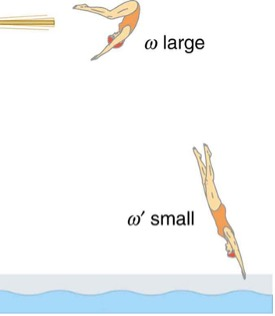
\includegraphics[width=4.5cm]{OS_10-33.jpg}
    \caption{OpenStax Figure 10.33.  The diver spins rapidly when curled up and slows when she extends her limbs before entering the water.}
    \label{OS10.33}
  \end{figure}
\end{myquestions}

\end{document}